% Atualizado para atender as normas ABNT por Mônica da Silva (04/11/2021)

% --- -----------------------------------------------------------------
% --- Elementos usados na Capa e na Folha de Rosto.
% --- EXPRESSÔES ENTRE <> DEVERÂO SER COMPLETADAS COM A INFORMAÇÂO ESPECÍFICA DO TRABALHO
% --- E OS SÌMBOLOS <> DEVEM SER RETIRADOS 
% --- -----------------------------------------------------------------
\autor{Thiago Augusto Fernandes de Carvalho} % deve ser escrito em maiúsculo

\titulo{Avaliação da fração de ejeção cardíaca em ecocardiogramas utilizando uma rede neural
UViT / Roberta}

\instituicao{UNIVERSIDADE FEDERAL FLUMINENSE}

\orientador{Flávio Luiz Seixas}


\local{NITER\'{O}I}

\data{2024} % ano da defesa

\comentario{Dissertação de Mestrado apresentada ao Programa de P\'{o}s-Gradua\c{c}\~{a}o em Computa\c{c}\~{a}o da \mbox{Universidade} Federal Fluminense como requisito parcial para a obten\c{c}\~{a}o do Grau de \mbox{Mestre em Computa\c{c}\~{a}o}. \'{A}rea de concentra\c{c}\~{a}o: \mbox{Ciência da Computação}} %preencha com a sua área de concentração

% --- -----------------------------------------------------------------
% --- Capa. (Capa externa, aquela com as letrinhas douradas)(Obrigatório)
% --- ----------------------------------------------------------------
\capa

% --- -----------------------------------------------------------------
% --- Folha de rosto. (Obrigatório)
% --- ----------------------------------------------------------------
\folhaderosto

% --- -----------------------------------------------------------------
% --- Ficha catalográfica obrigatória na versão final. (Obrigatório)
% --- ----------------------------------------------------------------



\begin{figure}[!ht]
    \centering
    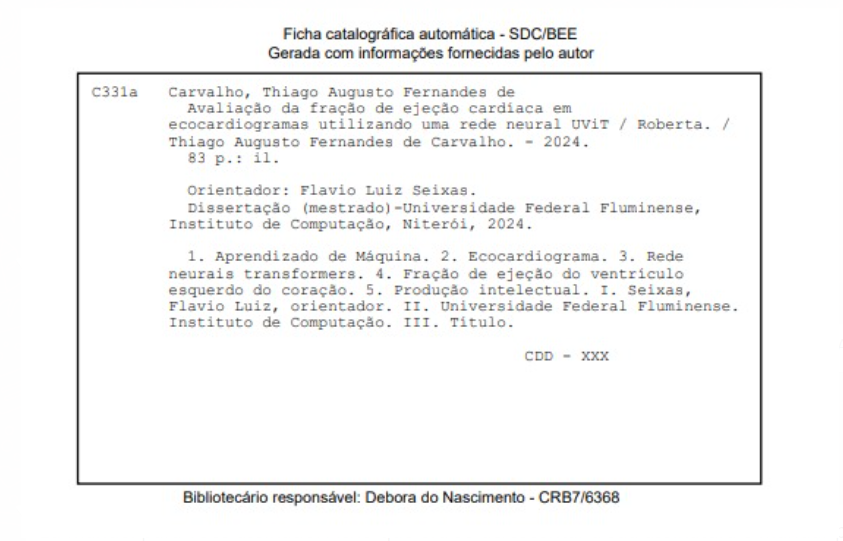
\includegraphics[width=1\linewidth]{capitulos//figuras/fichacarto.png}
    \caption{Ficha catalográfica}
    \label{fig:enter-label}
\end{figure}

\cleardoublepage


\pagestyle{ruledheader}
\setcounter{page}{1}
\pagenumbering{roman}

% --- -----------------------------------------------------------------
% --- Termo de aprovação. (Obrigatório)
% --- ----------------------------------------------------------------
\cleardoublepage
\thispagestyle{empty}

\vspace{-60mm}

\begin{center}
   {\large Thiago Augusto Fernandes de Carvalho}\\
   \vspace{7mm}

  Avaliação da fração de ejeção cardíaca em ecocardiogramas utilizando
uma rede neural UViT / Roberta.\\
  \vspace{10mm}
\end{center}

\noindent
\begin{flushright}
\begin{minipage}[t]{8cm}

Dissertação de Mestrado> apresentada ao Programa de P\'{o}s-Gradua\c{c}\~{a}o em Computa\c{c}\~{a}o da Universidade Federal Fluminense como requisito parcial para a obten\c{c}\~{a}o do \mbox{Grau} de  Mestre em Computa\c{c}\~{a}o. \'{A}rea de concentra\c{c}\~{a}o: \mbox{Ciência da Computação.} %preencha com a sua área de concentração

\end{minipage}
\end{flushright}
\vspace{1.0 cm}
\noindent
Aprovada em  Junho de 2024. \\

\begin{figure}[!ht]
    \centering
    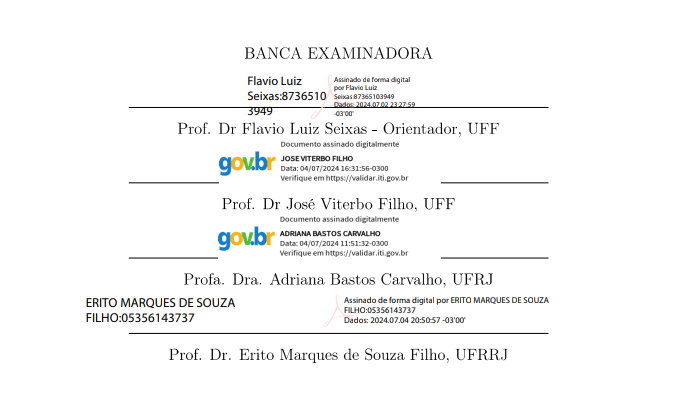
\includegraphics[width=1\linewidth]{capitulos//figuras/assinaturas.png}
    
    \label{fig:enter-label}
\end{figure}
\begin{center}
  \vspace{4mm}
  Niter\'{o}i \\
  %\vspace{6mm}
  2024

\end{center}



% --- -----------------------------------------------------------------
% --- Agradecimentos.(Opcional)
% --- -----------------------------------------------------------------
\pretextualchapter{Agradecimentos}
\hspace{5mm}


Agradeço primeiramente a Deus, pela força e pelas oportunidades únicas que me foram concedidas em minha jornada, e pelos momentos inestimáveis que tenho vivido. Expresso minha profunda gratidão ao meu orientador, pelo conhecimento transmitido, pelo suporte incansável, pelos conselhos sábios e pela paciência durante o desenvolvimento deste trabalho. Aos meus pais, pelo incentivo constante, pela crença inabalável em meu potencial e pelo amor e suporte que são a base de tudo que busco e conquisto. Vocês são minha inspiração e dedico a vocês cada passo que avanço. À minha esposa, companheira leal e fonte de amor e motivação diária. Sua presença é um suporte constante em minha vida, incentivando-me a alcançar meus sonhos e permanecer firme em meus objetivos. Seu apoio é inestimável, e esta conquista também pertence a você. À minha família, avós e tios, pelo afeto profundo e pelo suporte incondicional. Cada um de vocês tem um papel especial em minha vida, contribuindo para a minha felicidade e sucesso. Aos meus amigos e colegas, por serem uma rede de apoio, pelas risadas e momentos compartilhados. Cada um de vocês tem enriquecido minha vida de uma forma única. E a todos os professores e amigos que cruzaram meu caminho, em especial aos que se tornaram mentores e verdadeiros amigos, cujo apoio e incentivo foram cruciais para que eu alcançasse voos mais altos. Esta conquista também é de vocês.


% --- -----------------------------------------------------------------
% --- Resumo em português.(Obrigatório)
% --- -----------------------------------------------------------------
\begin{resumo}


Esta dissertação abordou a necessidade de diagnósticos cardíacos mais confiáveis, cruciais para tratamentos eficazes de diversas condições cardíacas, e focou na otimização de métodos de análise de ecocardiogramas para melhorar a precisão na estimativa da fração de ejeção do ventrículo esquerdo, essencial para diagnósticos cardíacos. Após uma revisão sistemática da literatura e a seleção de conjuntos de dados de ecocardiogramas adultos e pediátricos, a metodologia utilizou uma versão modificada da Ultrassom Video Transformer (UViT), integrando tecnologias como RoBERTa para análise espaço-temporal. A avaliação dos modelos, através de métricas como MAE, RMSE e R², revelou melhorias significativas em relação à bibliografia levantada, especialmente com o modelo RoBERTa, que se destacou em termos de precisão e capacidade de generalização para dados adultos e pediátricos. A pesquisa sugere que a abordagem proposta pode melhorar a precisão diagnóstica e ser aplicada clinicamente, contribuindo para decisões médicas mais informadas. As contribuições incluem um método robusto para análise de ecocardiogramas e abrem caminho para futuros trabalhos em categorização automática de pacientes por idade, melhoria da qualidade de imagens com redes neurais generativas e interpretação automática de relatórios médicos com modelos avançados de linguagem.

{\hspace{-8mm} \bf{Palavras-chave}}: ecocardiograma, fração de ejeção do ventrículo esquerdo, aprendizado profundo, análise de imagens médicas, RoBERTa, DistilBERT.

\end{resumo}

% --- -----------------------------------------------------------------
% --- Resumo em língua estrangeira.(Obrigatório)
% --- -----------------------------------------------------------------
\begin{abstract}

This dissertation addressed the need for more reliable cardiac diagnoses, crucial for effective treatments of various heart conditions, and focused on optimizing echocardiogram analysis methods to improve the accuracy of left ventricular ejection fraction estimation, which is essential for cardiac diagnoses. After a systematic literature review and the selection of adult and pediatric echocardiogram datasets, the methodology utilized a modified version of the Ultrasound Video Transformer (UViT), integrating technologies such as RoBERTa for spatiotemporal analysis. The evaluation of the models, using metrics like MAE, RMSE, and R², revealed significant improvements compared to the reviewed literature, especially with the RoBERTa model, which excelled in terms of accuracy and generalization capacity for both adult and pediatric data. The research suggests that the proposed approach can enhance diagnostic accuracy and be clinically applied, contributing to more informed medical decisions. The contributions include a robust method for echocardiogram analysis and pave the way for future work in automatic patient categorization by age, improving image quality with generative neural networks, and automatic interpretation of medical reports with advanced language models.

{\hspace{-8mm} \bf{Keywords}}: echocardiogram, left ventricular ejection fraction, deep learning, medical image analysis, RoBERTa.

\end{abstract}

% --- -----------------------------------------------------------------
% --- Lista de figuras.(Opcional)
% --- -----------------------------------------------------------------
%\cleardoublepage
\listoffigures



% --- -----------------------------------------------------------------
% --- Lista de tabelas.(Opcional)
% --- -----------------------------------------------------------------
\cleardoublepage
%\label{pag:last_page_introduction}
\listoftables
\cleardoublepage

% --- Lista de Abreviaturas e Siglas --------------------------------------------------
\begin{flushleft}
\textbf{Lista de Abreviaturas e Siglas}
\end{flushleft}

\begin{itemize}
    \item \textbf{BERT} - Bidirectional Encoder Representations from Transformers
    \item \textbf{CNN} - Redes Neurais Convolucionais (Convolutional Neural Networks)
    \item \textbf{DBN} - Redes de Crenças Profundas (Deep Belief Networks)
    \item \textbf{DistilBERT} - Distilled BERT
    \item \textbf{DPLAN} - Deep Pyramid Local Attention Network
    \item \textbf{E2D} - Ecocardiografia Bidimensional (Two-dimensional Echocardiography)
    \item \textbf{E3D} - Ecocardiografia Tridimensional (Three-dimensional Echocardiography)
    \item \textbf{EDNAS} - Pesquisa de Arquitetura Neural de Codificador-Decodificador (Encoder-Decoder Neural Architecture Search)
    \item \textbf{FEVE} - Fração de Ejeção do Ventrículo Esquerdo (Left Ventricular Ejection Fraction)
    \item \textbf{GAN} - Redes Adversárias Gerativas (Generative Adversarial Networks)
    \item \textbf{GPT-4} - Generative Pre-trained Transformer 4
    \item \textbf{IA} - Inteligência Artificial (Artificial Intelligence)
    \item \textbf{MAE} - Mean Absolute Error (Erro Médio Absoluto)
    \item \textbf{MLP} - Perceptrons Multicamadas (Multilayer Perceptrons)
    \item \textbf{NAS} - Pesquisa de Arquitetura Neural (Neural Architecture Search)
    \item \textbf{NLP} - Processamento de Linguagem Natural (Natural Language Processing)
    \item \textbf{R²} - Coefficient of Determination (Coeficiente de Determinação)
    \item \textbf{RBM} - Máquinas de Boltzmann Restritas (Restricted Boltzmann Machines)
    \item \textbf{RNA} - Redes Neurais Artificiais (Artificial Neural Networks)
    \item \textbf{RMSE} - Root Mean Square Error (Erro Quadrático Médio Raiz)
    \item \textbf{RoBERTa} - Robustly Optimized BERT Approach
    \item \textbf{RNN} - Redes Neurais Recorrentes (Recurrent Neural Networks)
    \item \textbf{SLR} - Revisão Sistemática da Literatura (Systematic Literature Review)
    \item \textbf{SOM} - Mapas Auto-Organizáveis (Self-Organizing Maps)
    \item \textbf{US} - Ultrassonografia (Ultrasound)
    \item \textbf{UViT} - Ultrasound Video Transformer
    \item \textbf{VE} - Ventrículo Esquerdo (Left Ventricle)
    \item \textbf{ViT} - Vision Transformer
\end{itemize}
\cleardoublepage
% -----------

% --- -----------------------------------------------------------------
% --- Sumario.(Obrigatório)
% --- -----------------------------------------------------------------

\pagestyle{ruledheader}
\tableofcontents
\pagebreak